\chapter{Prehľad}\label{chap:prehlad}

\section{Eclipse}

Informácie v tejto sekcii som čerpal z oficiálnej stránky Khronos Group \cite{fou}.

BlaBlaBlaBlaBla
Eclipse je platforma ktorá bola navrhnutá od základu pre budovanie integrovaného webu a nástroje na vývoj aplikácií. Platforma sama o sebe pre koncových užívateľov neposkytuje veľké množstvo funkcií. Jej hodnota je, že podporuje rýchly rozvoj integrovaných funkcií založených na rozšíreniach. Jadrom Eclipse je architektúra pre dynamické nachádzanie, načítavanie a chod rozšírení. 

\section{ADT}

Informácie v tejto sekcii som čerpal z oficiálnej stránky Khronos Group \cite{pro}.

ADT (Android vývojové nástroje) je rozšírenie pre vývojové prostredie Eclipse. ADT je navrhnuté tak aby poskytlo výkonné, integrované vývojové prostredie v ktorom sa dajú budovať Android aplikácie. ADT rozširuje možnosti vývojového prostredia Eclipse aby sa dali rýchlo nastaviť nové projekty, vytvárať užívateľské rozhranie aplikácie, pridávať balíky založené na Android rozhraniach pre programovanie aplikácií, ladenie aplikácie aj exportovanie .apk súborov za účelom distribúcie aplikácie.

\section{OpenGL ES}

Informácie v tejto sekcii som čerpal z oficiálnej stránky Khronos Group \cite{gro}.

OpenGL ES je voľné medziplatformové rozhranie pre programovanie aplikácií s plne funkčnou 2D a 3D grafikou na vstavané systémy vrátane konzol, telefónov, spotrebičov a vozidiel. Skladá sa z podmnožín knižnice OpenGL čím vytvára flexibilné a výkonné nízkoúrovňové rozhranie medzi softvérom a grafickou akceleráciou. OpenGL ES 1.X je pre hardvér s pevnou funkčnosťou a ponúka akceleráciu kvality obrazu a výkonu. OpenGL ES 2.X umožňuje plne programovateľnú 3D grafiku.

\section{jPCT-AE}

Informácie v tejto sekcii som čerpal z oficiálnej stránky jPCT \cite{ols}.

Rozhranie pre programovanie aplikácií jPCT-AE ponúka všetky funkcie potrebné na programovanie 3D hier a simulácií pre platformu Android. Rozhranie jPCT-AE je voľne prepojené s OpenGL ES.

\section{Presné vektorové textúry pre 3D vizualizácie v reálnom čase}

\subsection{Úvod}

V tejto sekcii by som chcel prezentovať jednu z metód vizualizácie v reálnom čase. Väčšina poznatkov z tejto sekcie sa opiera o informácie získané z článku  {\itshape Precise vector textures for real-time 3d rendering.} \cite{qmk08}

Svet okolo nás je plný povrchových vzorov s ostrými hranami. Ako sa k nim približujeme, tieto ostré hrany ostávajú ostré. Rastrové textúrové mapy, bežné prostriedky pre dekoráciu plôch v počítačovo generovanom zobrazovaní, nemajú túto vlastnosť. Keď približujeme textúrovanú plochu, táto plocha sa začne javiť rozmazaná alebo \textcolor{red}{pixelovaná} keď presiahneme rozlíšenie základnej textúrovej mapy. Táto metóda ponúka reprezentáciu vektorového obrázku dovoľujúcu aby bol použitý ako textúrová mapa, ktorá vyzerá ostro pri ľubovoľnom rozlíšení.

Prístupy pre priamu podporu určitých vektorových dát pri textúrovaní sa delia do dvoch hlavných kategórií:
\begin{itemize}
\item približné metódy
\item presné metódy
\end{itemize}
V oboch prípadoch, pre podporu textúrovania, táto reprezentácia musí podporovať efektívny ľubovoľný prístup. Anizotropné \textcolor{red}{vyhladzovanie} ktoré podporuje obrazové deformácie je tiež potrebné pre výsledky vo vysokej kvalite.

Približné metódy limitujú rozsah podporovaných vektorových obrázkov alebo akceptujú zníženú kvalitu obrázku výmenou za vyšší výkon. Príklady kompromisov približných metód zahŕňajú zaoblené rohy, obmedzená maximálna zložitosť v regióne, obmedzená podpora farieb a nakoniec podpora iba pre obmedzenú sadu oblých primitívnych typov.

V porovnaní, presné metódy vizualizujú obsah presne tak isto ako keď sú vyjadrené v štandardnom formáte vektorových obrázkov ako napríklad SVG. Výhoda vkladania obrázkov vyjadrených v štandardnej reprezentácií je, že na úpravu tohto obsahu môžu byť použité existujúce vektorové grafické nástroje a podpora plného rozsahu týchto nástrojov dáva maximálnu flexibilitu.

Bohužiaľ SVG a podobné súborové formáty ako PDF reprezentujú hranicu s parametrickými krivkami a \textcolor{red}{splinami} vyššieho rádu, ktoré komplikujú získavanie farby a vyhladzovanie. Rýchly ľubovoľný prístup a vysoko kvalitné vyhladzovanie vyžadujú rozšírenú reprezentáciu. Takéto rozšírené reprezentácie zvyčajne kombinujú štruktúru urýchľovača ktorá obmedzuje \textcolor{red}{okrajové vlastnosti} aby bola braná do úvahy pre každý prístup s reprezentáciou tých vlastností ktoré umožňujú efektívne vyhladzovanie.

Táto metóda vizualizácie prispieva k druhej kategórií prístupov pre priamu podporu určitých dát pri textúrovaní. Počíta presnú geometriu vo vektorovom obrázku ako je reprezentovaná v SVG súbore a vizualizuje ju s vysoko kvalitným vyhladzovaním.

Používa \textcolor{red}{podpísanú} vzdialenosť k najbližšej okrajovej vlastnosti ako implicitnú reprezentáciu tejto vlastnosti. Po vypočítaní, funkcia podpísanej vzdialenosti môže byť zmapovaná cez \textcolor{red}{smooth} krok k získaniu funkcie \textcolor{red}{splývania} pre vyhladzovanie a \textcolor{red}{spád} môže byť použitý k prispôsobeniu šírky prechodu k získaniu anizotropného vyhladzovania. Táto vzdialenosť môže byť tiež použitá k vizualizácii ťahov presnej šírky a k realizovaniu špeciálnych efektov ako razba.

Okraje v štandardných súborových formátoch vektorovej grafiky ako napríklad SVG môžu zahrňovať body, úsečky, eliptické oblúky a spline krivky. K týmto okrajovým prvkom bude referované ako k vlastnostiam. Z týchto vlastností \textcolor{red}{priestorové} spline krivky sú tie najzložitejšie. Priame počítanie vzdialenosti k parametrickým spline krivkám vyššieho rádu je nákladné.

\subsection{Algoritmus}

Algoritmus sa skladá z dvoch častí. Z predspracovanej reprezentácie vkladaním vektorového obrázka do množiny textúrových máp a z algoritmu realizovanom v \textcolor{red}{shaderi} pre podanie tejto informácie k vypočítaniu farby tohto vektorového obrázku v ľubovoľnom bode. Táto reprezentácia musí podporovať rýchly prístup k minimálnemu množstvu dát v každom bode. Základom výpočtu farby je rýchly výpočet vzdialenosti.

Za účelom vybudovania tejto reprezentácie sa najskôr vektorový obrázok prekryje rovnomernou mriežkou. Každá bunka sa skontroluje aby sa našla podmnožina okrajových vlastností ktoré ju pretínajú. Všetky okrajové vlastnosti ktoré pretínajú nejakú bunku sa uložia do zoznamu pre jednotlivé bunky. Tento zoznam je potom rozšírený o vlastnosti mimo bunky do určitej vzdialenosti pre podporu vyhladzovania.

Získavanie farby a vyhladzovanie okrajov pre ľubovoľný bod v bunke stačí brať do úvahy iba zoznam vlastností bunky. 

\subsection{Predspracovanie}

Typický SVG obrázok je zložený z uzavretých ciest alebo ťahov. Cesty môžu mať okraje rôznych šírok a farieb a môžu byť orientované aj do smeru alebo protismeru hodinových ručičiek. Región uzavretý do cesty môže byť vyplnený jednou farbou alebo spádom. Ťahy môžu mať taktiež farbu a šírku. 

Aby sme vytvorili danú reprezentáciu musia sa najskôr všetky krivky rozdeliť do jednotvárnych úsekov čo neskôr zjednoduší výpočet vzdialenosti.

\subsubsection{Delenie kriviek}

\begin{figure}[H]
\begin{center}
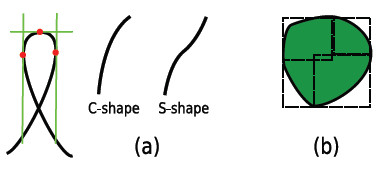
\includegraphics[width=0.7\textwidth]{images/splitting_curves_1}
\caption{(a) Všetky krivky sa rozdelia do vlastností tvarov C a S v každom bode kde sú dotyčnice horizontálne alebo vertikálne. (b) Okrajový rámček cesty je okrajovým rámčekom pre jej vlastnosti. \cite{qmk08}}
\label{img:splitting_curves_1}
\end{center}
\end{figure}
Pre zjednodušenie výpočtu vzdialenosti sa každá krivka v bodoch kde ich dotyčnica je horizontálna alebo vertikálna rozdelí. Na príklad na Obr. \ref{img:splitting_curves_1}(a) sa daný spline v červených bodoch rozdelí na štyri úseky. Nech je parametrický zápis krivky daný \( P\big(u\big) = [x\big(u\big),y\big(u\big)]\). Deliace body \(u*\) pre priestorové spliny sú dané riešením koreňov kvadratických parametrických splinov dosadením komponentov dotyčnice \(\overrightarrow{T}\big(u\big) = [x'\big(u\big),y'\big(u\big)]\) of \(P\big(u\big):\)
\begin{center}
\(x'\big(u*\big) = 0\) or \(y'\big(u*\big) = 0\).
\end{center}
Existujú najviac štyri deliace body keďže existujú najviac dve riešenia pre vyššie uvedené rovnice, takže krivky sú rozdelené do najviac piatich úsekov.

Každý výsledný úsek má jednoduchý tvar. Po delení sú možné iba dva druhy tvarov ako je ukázané na Obr. \ref{img:splitting_curves_1}(a). Tieto tvary sa budú nazývať C-tvary a S-tvary. Treba si všimnúť, že nad každým úsekom, \(x'\big(u\big)\) a \(y'\big(u\big)\) sú buď úplne pozitívne alebo negatívne. Takéto funkcie sa budú nazývať jednotvárne. C-tvar reprezentuje všetky krivky bez inflexného bodu. S-tvar reprezentuje všetky krivky s jedným inflexným bodom. Kedže druhá derivácia priestorovej funkcie je lineárna funkcia, existujú najviac dva také body: jeden pre \(x''\big(u*\big) = 0\) a jeden pre \(y''\big(u*\big) = 0\).

\subsubsection{Zisťovanie vlastností prekrývajúcich bunku}

Za účelom vybudovania štruktúry urýchľovača sa najskôr vektorový obrázok prekryje rovnomernou mriežkou. Pre každú bunku sa zistí ktoré cesty obsahujú celú bunku a ktoré cesty ju pretínajú.

Pre každú bunku je tento proces robený v poradí vykresľovania cesta po ceste. Poradie vizualizácie vo vektorových obrázkoch je dôležité a súčasťou predspracovania je tiež riešenie viditeľnosti.

Pre urýchlenie tejto procedúry sa vypočíta okrajový rámček každej cesty, zarovnaný podľa osi. Ak bunka neprekrýva tento okrajový rámček cesty, tak táto cesta nemôže pokryť bunku ani prejsť jej okrajom. Keďže všetky rozdelené vlastnosti sú jednotvárne, okrajová mriežka pre každú z nich sa dá vytvoriť z jej dvoch koncových bodov. Okrajová mriežka pre celú cestu môže byť vypočítaná pomocou okrajových mriežok jej vlastností ako je ukázané na Obr. \ref{img:splitting_curves_1}(b).

Ak okrajová mriežka cesty prekrýva bunku tak sa skontrolujú všetky vlastnosti cesty s bunkou. Jednotvárne vlastnosti sa môžu pretínať so štyrmi okrajovými čiarami bunky použitím klasických numerických metód. Ak vlastnosť pretne nejaký okraj alebo ak je úplne obsiahnutý bunkou, tak sa uloží do zoznamu bunky.

Ak žiadna vlastnosť cesty neprekrýva bunku, sú možné dve situácie. A to, že cesta môže byť mimo bunku alebo bunka obsahuje úplnú cestu. Ak ide o druhý prípad, všetky vlastnosti ktoré sú uvedené v zozname bunky sa vymažú a farba pozadia bunky sa nastaví na farbu výplne aktuálnej cesty. Všetky predošlé vlastnosti budú prepísané touto novou cestou.

\subsubsection{Rozšírenie bunky}

Keď je cesta skontrolovaná s bunkou, musí sa zväčšiť rozsah bunky na toleranciu nejakej úrovne textúrovej \textcolor{red}{minifikácie}. Vyhladzovací filter bude mať určitú šírku a je potrebné aby sa vedeli počítať vzdialenosti aspoň na takúto šírku. Rozsah tohto rozšírenia závisí na úrovni minifikácie obrázka ktorá má byť podporovaná počas vektorovej vizualizácie.

Pri vyšších úrovniach minifikácie, vizualizácia textúr by mala byť realizovaná pomocou rastrovo založenej MIP mapy. Tento rastrový obrázok môže byť vizualizovaný priamo z vektorovej textúry. Pod minifikáciou MIP mapovanie presnú vyhladenú reprezentáciu vektorového obrázku a prechody môžu byť zvládnuté použitím alpha kanálu rastrovej textúry. Rastrové obrázky s najlepším rozlíšením by mali byť uložené s \(\alpha = 0\), ostatné hrubšie úrovne by mali používať \(\alpha = 1\). Potom trilineárna interpolácia z \(\alpha\) dá správnu hodnotu pre splynutie medzi rastrovou a vektorovou vizualizáciou. Vizualizácia vektorov môže byť blokovaná požitím riadeného toku v shaderi keď \(\alpha = 1\). Ak textúra obsahuje priehľadnosť, potom shader môže vypočítať prechodovú funkciu výlučne použitím Jacobiana súradníc tejto textúry na priestorové mapovanie obrazovky.

Avšak rozširovanie bunky pevnou hodnotou nemusí zahrnúť všetky vlastnosti potrebné na správny výpočet vnútorného/vonkajšieho testu. Šírka rozšírenia by mala byť určená tak, že keď je pridaná vlastnosť križujúca bunku, mali by byť zahrnuté taktiež všetky vlastnosti ktoré by mohli byť bližšie pre ktorýkoľvek bod v bunke.

\subsubsection{Štruktúra urýchľovača}

V tomto momente máme zoznam dôležitých vlastností a farbu pozadia každej bunky. Tieto informácie musia byť uložené v štruktúre urýchľovača. Metóda používa tri textúry na efektívne uloženie týchto informácií.

\begin{figure}[H]
\begin{center}
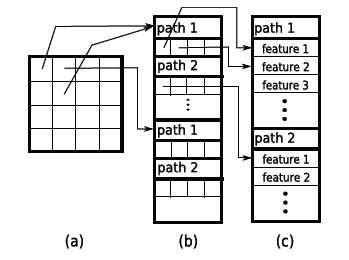
\includegraphics[width=0.7\textwidth]{images/acceleration_structure_1}
\caption{Používajú sa tri textúry na uloženie štruktúry urýchľovača. \cite{qmk08}}
\label{img:acceleration_structure_1}
\end{center}
\end{figure}

Na najnižšej úrovni sa uvádzajú všetky vlastnosti všetkých ciest vrátane bodov, úsečiek, priestorových splinov, elíps a tak ďalej v jednej textúre. Každá vlastnosť je uložená iba raz. Vlastnosti sú zoskupené a triedené podľa ciest. Vlastnosti patriace tej istej ceste sú dané dohromady s hlavičkou ktorá ukladá informácie jednej cesty. Táto textúra je ukázaná na Obr. \ref{img:acceleration_structure_1}(c).

Pre každú bunku, zoznam vlastností križujúcich túto bunku sú triedené podľa ciest ku ktorým patria. Táto textúra má uložené smerníky do textúry nižšej úrovne ktoré ukazujú na použité vlastnosti. Je teda potrebný iba jeden úložný priestor pre každú vlastnosť. Táto fáza je ukázaná na Obr. \ref{img:acceleration_structure_1}(b).

Posledná textúra je mriežková textúra zodpovedajúca bunkám. Pre každú bunku uchováva začiatočné umiestnenie zoznamu vlastností v druhej textúre. Zodpovedajúci zoznam vlastností sú presne tie ktoré bunku prekrývajú. Taktiež uchováva počet ciest ktoré prechádzajú cez túto bunku a farbu pozadia pre bunku. Ak majú dve bunky rovnaký zoznam vlastností tak zdieľajú jediný zoznam v zozname textúr opísanom vyššie.

\subsection{Shaderový výpočet}

Shaderový výpočet pristupuje k urýchľovaču aby rozhodol ktoré vlastnosti je potrebné brať do úvahy pre každú bunku. Postupne je zvážená každá cesta a zložená jej farba pre vytvorenie konečnej farby.

\subsubsection{Skladanie cesty}

Poradie ciest a vlastností v každej bunke musí súhlasiť so vstupným poradím v SVG súbore. Začína sa s farbou pozadia a zoznamom ciest a vlastností bunky. V každej ceste sa postupne vypočíta podpísaná vzdialenosť k najbližšej vlastnosti. Pre každú cestu sa použije toto znamienko aby sa zistilo či testovací bod leží vnútri alebo vonku tejto cesty. Bod je vnútri cesty ak sa nachádza na pravej strane od najbližšej vlastnosti a v tomto prípade sa bude používať negatívna vzdialenosť. Najbližšia vzdialenosť každej novej cesty môže mať rovnaké alebo iné znamienko ako predchádzajúca a môže byť tiež menšia alebo väčšia v rozmere.

Vždy sa sleduje vzdialenosť \(d\) s najmenším rozmerom, farba popredia \(F\) a farba pozadia \(B\). Tieto dve farby sú vždy tie farby ktoré sa nachádzajú na každej strane najbližšieho okraja. Predpokladajme, že \(D\) je najbližšia podpísaná vzdialenosť k nasledujúcej ceste v postupnosti a \(C\) je farba jej výplne. Obnovenie \(d\), \(F\) a \(B\) prebehne nasledovne:
\begin{displaymath}
\begin{array} {l}
\text{bool } q = D < 0 \text{ alebo } |D| < |d|\text{;} \\
\text{bool } p = q \text{ and } d < 0; \\
B = p \text{ ? } F : B\text{;} \\
F = q \text{ ? } C : F\text{;} \\
d = q \text{ ? } D : d\text{;}
\end{array}
\end{displaymath}
Na konci tohto procesu sa vzdialenosť s najmenším rozmerom a jej znamienko použijú k nájdeniu hodnôt splývania pre vyhladzovanie použitím smooth kroku so šírkou prechodu použitím Jacobiana súradnicovej transformácie textúry.
\begin{figure}[H]
\begin{center}
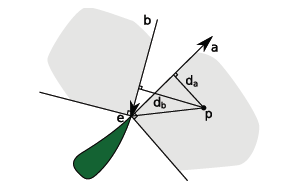
\includegraphics[width=0.7\textwidth]{images/path_compositing_1}
\caption{Chyby vnútorného/vonkajšieho testu v rohoch. \cite{qmk08}}
\label{img:path_compositing_1}
\end{center}
\end{figure}

Keď sa používa podpísaná vzdialenosť na zistenie či bod leží vnútri alebo vonku cesty, v ostrých rohoch môže nastať nejednoznačnosť. Na Obr. \ref{img:path_compositing_1}, sa nachádza cesta reprezentovaná zeleným útvarom. Priamky \(be\) a \(ea\) sú dotyčnicami na \textcolor{red}{roh} \(e\). Smery týchto priamok súhlasia so smerom obrysu cestu. Pre ľubovoľný bod nachádzajúci sa v šedej vyfarbenej ploche platí, že jeho najbližšia vzdialenosť k okraju cesty je vzdialenosť k tomuto rohu. Na tomto obrázku, najbližšia vzdialenosť bodu \(p\) k ceste je \(pe\). Ak sú dve najbližšie vzdialenosti rovnaké jednoduché pravidlo najmenšej vzdialenosti náhodne vyberie buď priamku \(be\) alebo priamku \(ea\) na vnútorný/vonkajší test. Znamienko sa vypočíta premietnutím \(pe\) na zodpovedajúcu dotyčnicu zarotovanú o 90 stupňov.

\subsubsection{Výpočet vzdialenosti}

Jadro tohto algoritmu je výpočet podpísanej vzdialenosti k vlastnosti. Výpočet vzdialenosti k úsečke je jednoduchý. Avšak výpočet vzdialenosti ku kvadratickým alebo priestorovým splinom alebo eliptickým oblúkom je zložitejší. Nasledujúci postup výpočtu vzdialenosti je založený na binárnom vyhľadávaní a môže byť uplatnený na akúkoľvek parametrickú krivku.
\begin{figure}[H]
\begin{center}
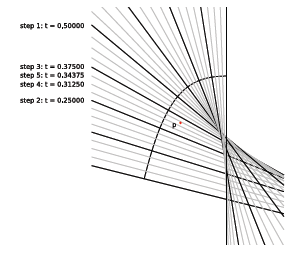
\includegraphics[width=0.7\textwidth]{images/distance_computation_1}
\caption{Najbližší bod na krivke k ľubovoľnému bodu p sa dá nájsť použitím binárneho vyhľadávania založenom na preverení normály priamky. V regiónoch kde sa normálové priamky pretínajú, môže byť algoritmus neúspešný ale normálové priamky sa navzájom pretínajú iba za najmenším zakrivením polomeru. \cite{qmk08}}
\label{img:distance_computation_1}
\end{center}
\end{figure}

Najprv sa ohraničí parametrické umiestnenie najbližšieho bodu na ceste použitím intervalu ktorý obsahuje celý úsek krivky. Pri každej iterácií je tento interval rozdelený v jeho parametrickom stredovom bode. Potom sa predĺži normála v deliacom bode do deliacej roviny ako je ukázané na Obr. \ref{img:distance_computation_1}. Tento bod sa overený s touto rovinou. Polovica krivky ktorá je na tej istej strane roviny ako tento bod sa vyberie pre nasledujúcu iteráciu. Iterácie sa môžu opakovať až dokým sa nedosiahne určitá chybová tolerancia alebo po daný počet iterácií.
\begin{figure}[H]
\begin{center}
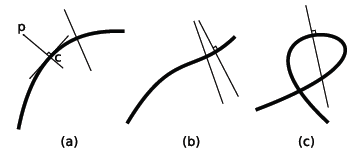
\includegraphics[width=0.7\textwidth]{images/distance_computation_2}
\caption{Normálové priamky C-tvarových a S-tvarových kriviek túto krivku znovu nepretínajú. \cite{qmk08}}
\label{img:distance_computation_2}
\end{center}
\end{figure}

Pre porozumenie vlastností tohto algoritmu si najskôr treba všimnúť, že normálové priamky C-tvarov a S-tvarov pretínajú krivku vždy iba raz, Obr. \ref{img:distance_computation_2}(a),(b). Prípad (c) nenastane keďže sú krivky rozdelené. Potom si treba všimnúť ak nakreslíme dve normálové priamky v ľubovoľných bodoch na krivke, tak sa tieto normálové priamky nikdy nepretnú na konvexnej strane krivky. Avšak vždy sa pretnú na konkávnej strane ale vo vzdialenosti ktorá je vždy väčšia ako najmenšie zakrivenie polomeru na krivke. Preto pre všetky body na konvexnej strane a pre body v rozsahu polomeru zakrivenia na konkávnej strane, normálové priamky zavádzajú sekvenčné usporiadanie na priestor v okolí krivky. Binárne vyhľadávanie určí polohu bodov procesu v tomto poradí.